\section{Control for Simulation Experiments}
In \cref{sec:control_sim}, in order to assess potential benefits of using the
neuromuscular model for prosthesis control, we perform simulated experiments of
an amputee walking with a powered knee and ankle prosthesis. In those
experiments, to generate the reference torques for the SEAs, we use a hybrid
neuromuscular control that blends the muscle based stance-control
(\cref{sec:neuro_stance_reflexes}) with the idealized swing leg placement
control \cref{sec:neuro_swing_reflexes}. 

For the stance control of the prosthesis, we utilize only muscles and reflexes
of the lower leg: the Hamstring, Vastus, Gastrocnemius, Soleus, and Tibialis
Anterior. These muscles are stimulated by
\crefrange{eq:sol_stim}{eq:ham_stim_full}. However, because the hamstring muscle
spans the hip joint as well, and we do not wish to instrument the torso of the
amputee user, we assume that the torso angle remains fixed at $\phi_\tn{ref}$, 
thereby reducing the hamstring stimulation to \cref{eq:ham_stim}.

Additionally, we make make two modifications to the prosthesis-side swing leg
control. First, on the prosthesis-side hip we remove the feed-forward term that
neutralizes the disturbance created by the knee's stop and extend phase
(\cref{eq:hipfeedforward}), requiring that feedback control deal with this
torque.  Second, we do not use the adaptive leg placement policy of the swing
control (\cref{eq:simbicon}) as the prosthesis does not have access to
information about the amputee's center of mass and stance leg ankle position.
Instead the prosthesis swing leg control employs a constant target leg angle,
$\alpha_\tn{tgt} = \mathrm{const}$.

The torques produced by the swing controller augment the net torques produced by
the Hill-type muscles and reflexes during stance. At heel strike, the control
policy switches from using the swing leg control torques to the stance torques
generated by the muscle models. In late stance, the policy mixes the torques
specified by the stance and swing controllers by scaling the stance and swing
torques and muscle stimulations in proportion to the normalized ground reaction
force,
\begin{align}
    \tau_\textrm{late stance} &= \tau_\tn{stance}(GRF) +
    \tau_\tn{swing}(1 - GRF), \label{eq:stance_grf_trans}\\ 
    S^\tn{m}_\textrm{late stance}  &= S^\tn{m}(GRF).\label{eq:swing_grf_trans}
\end{align}
During swing, only the swing leg torques are used.

\section{Control for Prosthesis Experiments}\label{sec:nm_control_prosthesis}

\begin{figure*}[htb]
    \centering
    \includegraphics[width=0.9\textwidth]{pros_and_nm_model}
    \caption[Interaction between transfemoral prosthesis and neuromuscular
    control]{(a) Custom transfemoral prosthesis with series elastic actuators.
    In experiments in this thesis, we use an adaptor to test the prosthesis with
    able-bodied subjects. (b) During stance, we propose a control based on a
    neuromuscular model of human physiology that generates joint torques through
    virtual muscles that are stimulated by hypothesized local reflex
    pathways.}\label{fig:pros_and_nm_model}
\end{figure*}

In \cref{sec:preference_optimization,sec:nm_vs_imp,sec:phase_estimation} we
perform experiments with the prosthesis hardware (detailed in
\cref{sec:pros_design}) with the neuromuscular model control. To operate this
control on the prosthesis, we measure the prosthesis' joint angles using its
onboard encoders, the user's thigh angle using an inertial measurement unit, and
ground reaction signals via hall effect sensors embedded in the foot. The
measured joint angles feed into the muscle and reflex models in order to
calculate the desired joint torques for the prosthesis, which are then achieved
by the low-level SEA control~(\cref{sec:sea_control}). We use the ground
reaction forces in 

In \cref{sec:nm_vs_imp,sec:phase_estimation}, the stance control follows the
equations given in \cref{sec:neuro_stance_reflexes} with the same modifications
to the Hamstring as were made for the simulated experiments $(\phi_\tn{hip} =
\phi_\tn{ref})$. In \cref{sec:preference_optimization} we experiment with an
augmented version of the model that contains a Biceps Femoris Short Head, a
monoarticular knee flexor (see \cref{fig:pros_and_nm_model}). This muscle helps
prevent knee over extension via length feedback of the form
\begin{align}
    \func{S}[][\tn{bfsh}]{t} &= S_0^\tn{bfsh} + G_\tn{bfsh}^\tn{bfsh}
        \func{L}[\tn{bfsh}][]{t_\tn{l}}\label{eq:bfsh_stim}.
\end{align}
In this model, knee over extension is further prevented by inhibiting the vastus
in proportion to the BFsH length. Consequently, the vastus stimulation becomes 
\begin{align}
\func{S}[][\tn{vas}]{t} &= S_0^\tn{vas} 
    + G_\tn{vas}^\tn{vas} \func{F}[\tn{vas}][]{t_\tn{m}} 
    - G_\tn{vas}^\tn{bfsh} \func{L}[\tn{bfsh}][]{t_\tn{m}}.
    \label{eq:vas_stim_w_bfsh}
\end{align}
The properties of BFsH muscle (as well the properties of the other muscles) are
based on human physiological parameters described in \citet{song2015neural}.

While our simulated experiments used the idealized reflexive swing control
described in \cref{sec:neuro_swing_reflexes}, in our prosthesis experiments we
instead use the minimum-jerk trajectory swing controller proposed by
\citet{lenzi2014speed}, which automatically adapts to walking speed and produces
human-like trajectories. In our implementation, at every toeoff the control method
generates a pair of minimum jerk trajectories for each joint: one that starts at
the toeoff angle, velocity and acceleration and reaches peak knee flexion or
ankle dorsiflexion and another that goes from the peak flexion state to the heel
strike state. The knee and ankle joints are set to \unit[65 and 2]{deg} at peak
flexion and \unit[2 and -5]{deg} at heel strike respectively. The prosthesis
then follows these desired joint angles via proportional/derivative feedback
plus a model-based feedforward term. Combined, the feedback and feedforward
terms specify the desired joint torques which the low-level SEA control tries to
achieve (\cref{sec:sea_control}). The use of the feed forward term and SEA
torque control during swing allows the system to maintain a level of impact
compliance despite following a trajectory.

The swing phase duration is set to 60\% of the previous stance phase duration.
In the \cref{sec:preference_optimization,sec:nm_vs_imp}, we specified that the
peak flexion angles for both the knee and ankle would be achieved simultaneously
at 25\% of swing. Later, in the work presented
\cref{sec:trip_avoidance,sec:phase_estimation}, we delayed peak ankle flexion to
50\% of swing to help avoid some of the frequent trips during swing that we
discovered during the experiment presented in \cref{sec:nm_vs_imp}.
\Cref{sec:trip_avoidance} also presents a more principled approach to avoiding
these swing trips that explicitly predicts and plans to avoid premature foot
contact with the ground.

We switched to this minimum jerk trajectory swing control approach for two
reasons: First, preliminary experiments with the idealized swing control on the
prosthesis hardware revealed that it was more sensitive to errors in the torque
control. This seemed especially true in the second phase of the idealized swing
control, in which small damping torques are used to control the rate of
extension of the knee. In our SEA design (\cref{sec:pros_mech_design}), small
errors in the torque measurement can build up over time due to encoder shift and
thermal expansion.  While these torque errors are insignificant during stance,
they appeared to affect the behavior of idealized swing control. In contrast, a
trajectory based approach can compensate for these errors through its explicit
position feedback. Second, in our simulated experiments, we held the target
angle $\alpha_\tn{tgt}$ constant. However, in a real system, the target angle
prediction should adapt to specific users and to variations in speed, terrain,
and balance recovery intent. How best to predict this target angle remains an
open research question and is not addressed in this thesis.

\begin{marginfigure}
    \centering
    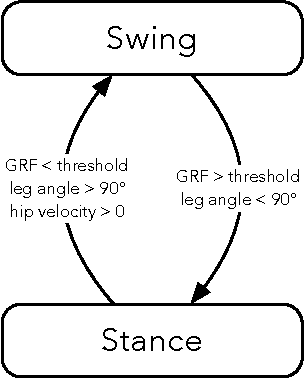
\includegraphics[width=\linewidth]{stance_swing_state_machine}
    \caption[Universal stance/swing state machine]{Universal stance/swing state
    machine utilized for all hardware
    experiments.}\label{fig:stance_swing_state_machine}
\end{marginfigure} 
To switch between stance and swing phases, the prosthesis follows the state
machine depicted in~\cref{fig:stance_swing_state_machine}.  Transitions to
stance occur when the leg is ahead of the frontal plane (leg angle $\alpha >
90^\circ$, see \cref{fig:swing_leg_polar}) and when the ground reaction force
(GRF) exceeds a hand-tuned threshold. Transitions to swing are allowed when the
GRF falls below a threshold, the foot is behind the frontal plane $(\alpha <
90^\circ)$, and the hip is flexing. For the experiments described in
\cref{sec:preference_optimization,sec:nm_vs_imp,sec:trip_avoidance} we use the
prosthesis' built-in GRF sensors detailed in \cref{sec:mech_design_grf}. In
later work (\cref{sec:phase_estimation}), involving stepping on objects, we use
the GRF readings from an instrumented treadmill, as they proved more reliable in
this disturbed case.
